\documentclass{article} % for short documents
%\documentclass{report} % for longer documents


%% Defining the language for the document
\usepackage[english]{babel}
\usepackage[english]{isodate}
\usepackage{wrapfig}
\usepackage{imta_core}
\usepackage{imta_extra}
\setcounter{secnumdepth}{3}
% !TeX spellcheck = fr_FR
\usepackage{listings}
\usepackage{xcolor}
\usepackage{amsfonts} 

\definecolor{codegreen}{rgb}{0,0.6,0}
\definecolor{codegray}{rgb}{0.5,0.5,0.5}
\definecolor{codepurple}{rgb}{0.58,0,0.82}
\definecolor{backcolour}{rgb}{0.95,0.95,0.92}

\lstdefinestyle{mystyle}{
	backgroundcolor=\color{backcolour},   
	commentstyle=\color{codegreen},
	keywordstyle=\color{magenta},
	numberstyle=\tiny\color{codegray},
	stringstyle=\color{codepurple},
	basicstyle=\ttfamily\footnotesize,
	breakatwhitespace=false,         
	breaklines=true,                 
	captionpos=b,                    
	keepspaces=true,                 
	numbers=left,                    
	numbersep=5pt,                  
	showspaces=false,                
	showstringspaces=false,
	showtabs=false,                  
	tabsize=2
}

\lstset{style=mystyle}


%% Addtionnal packages can be loaded here
% \usepackage{biblatex} % for a complete and flexible bibliography


\cleanlookdateon % formats date according to the loaded language from now on

%% General informations
\author{Alexandre ALLANI}
%\imtaAuthorShort{<author's initials>}
\imtaSuperviser{Encadrant : Jean PRUVOST, consultant en datascience \\
Conseiller d'étude : Romain BILLOT \\
Responsable filière : Cécile BOTHOREL}

\date{\noexpand\today} % automatically print today's date, can be redefined using \date{<date>}
\title{Rapport de stage de fin d'étude}
\subtitle{Consultant en datascience chez Sia Partners}
%\imtaVersion{<version>}

%Add extra other companies' logo
%If needed, options can be passed to the underlying \includegraphics by calling \imtaAddPartnerLogo[<options>]{<path>}
\imtaAddPartnerLogo{sia_logo.jpg}


\imtaSetIMTStyle % Sets font and headers/footers according to the IMT Atlantue style guidelines


%%%%%%%%%%%%%%%%%%%%%%%%%%%%%%% 
%%%%%%%%%% BEGINNING %%%%%%%%%% 
\begin{document}

% front cover
\imtaMaketitlepage

\section{Résumé}
\newpage

\section{Summary}
\newpage



\tableofcontents
\newpage


\section{Introduction}
\newpage

\section{Présentation de l'entreprise}
\newpage

\section{Mission : webscrapping pour Cleep (1 mois)}
Cette partie est consacrée à la première mission que j'ai effectué sur le sujet du webscrapping pour Cleep. Le webscrapping est la collecte de données/informations sur des sites internet via un ou plusieurs scripts. Le but sera alors principalement de "piocher" dans le code source du site internet à webscrapper, ou via les requêtes effetuées par le serveur, les données que l'on souhaite récupérer.\\ \\
Cette mission mêle à la fois des problématiques de récupérations de données, mais aussi d'automatisation de webscrapping via certains algorithmes que j'ai développé.

\subsection{Présentation de Cleep}

Cleep est une start-up créée en 2017, développant une application éponyme sur le sujet de l'achat en ligne. L'application permet de sauvegarder un produit repéré sur un site marchand quelconque (que ce soit un site généraliste comme Amazon ou un site spécialisé comme Asos). 
\begin{wrapfigure}[14]{r}{0.5\textwidth}
	\begin{center}
		
\includegraphics[keepaspectratio = true,scale=0.2]{cleep.jpg}
	\end{center}
	\caption{Logo de Cleep}
\end{wrapfigure}
Cette application mobile est disponible sur mobile (iOS \& Android) mais aussi via un site Internet \cite{cleep}. Le principe de l'application est de pouvoir enregistrer n'importe quel produit pour ensuite le retrouver dans l'application. Il est alors possible de consulter via cette dernière le prix, la description, le nom, le site d'origine ainsi que les images reliés à ce produit. Le but de l'application est donc de faciliter l'achat de produits en ligne en ne passant que par une seule et unique plateforme. Par ailleurs, il est possible de créer une liste de "Cleep" (ie de produit) et de partager ces listes. Les listes publiques peuvent être trouvées via le moteur de recherche intégré. \\
Sia Partners a investi 400000€ dans Cleep fin 2018, et travaille en collaboration sur différents sujets, notamment en matière de datascience. En plus du côté simplification du shopping en ligne, Cleep avec ses listes et son moteur de recherche permet de suivre des listes plus ou moins influentes. Ainsi l'application permet de se tenir au courant des modes actuelles et de celles à venir. Cela explique l'investissement de Sia Partners.\\
Vocabulaire spécifique à Cleep :
\begin{itemize}
	\item cleep : Produit en ligne, enregistré dans la base de donnée. Un cleep est composé d'un prix, des images associés au produit, d'une description, du nom du produit ainsi de du site internet d'origine.
	\item liste de Cleep : Liste de Cleep, pouvant être partagé entre plusieurs utilisateurs. Chaque cleep est enregistré dans une liste.
	\item cleeper : Action d'enregistrer un produit dans l'application
\end{itemize}

J'ai travaillé pendant près de 3 mois pour Cleep. Je communiquais principalement avec Damien Meurisse côté Cleep et Paul Saffer côté Sia Partners.J'ai travaillé sur deux sujets :
\begin{itemize}
	\item Webscrapping : Acquisition et traitement des données. Cela est fondamental pour le fonctionnement de Cleep
	\item Moteur de recommandation. Avant mon arrivé, aucun moteur de recommandation n'existait. Cette fonctionnalité était de plus en plus nécessaire afin que l'utilisateur puisse chercher de nouveau cleeps autrement que par le moteur de recherche présent dans l'application.
\end{itemize}
\newpage
\subsection{Objectifs et problématique}
Cleep est une application reposant sur les articles et produits qu'elle permet d'enregistrer, mais aussi sur les méta-données qui leurs sont reliés. En effet, en allant sur Cleep, l'utilisateur doit pouvoir retrouver l'ensemble des informations qu'il recherche, sans pour autant retourner sur le lien de l'article. Il existe deux moyens d'enregistrer un produit :
\begin{itemize}
	\item Par capture d'écran du site : l'image est enregistré dans l'application. L'utilisateur peut alors renseigner lui même les informations dont il a besoin (ie le prix, le nom de l'article, etc.). Le cleep créé est composé de la capture d'écran et des informations renseignés.
	\item Avec le lien du site : Grâce à un procédé, détaillé plus tard, le produit avec ses images et ses méta-données sont cleepés.
\end{itemize}
En général l'enregistrement via capture d'écran n'est pas optimal pour l'application. En effet, les utilisateurs prennent rarement le temps d'enregistrer toutes les informations, ce qui les intéresse en priorité est de garder l'image et le nom du produit dans l'application afin d'avoir un souvenir de ce dernier. Le cleep ainsi enregistré n'est pas utile pour Cleep car manquant de beaucoup d'informations.\\
En effet, Cleep possède une base de donnée dans laquelle les produits sont enregistrés avec leur méta-données. Un produit est composé des éléments suivant :
\begin{itemize}
	\itemsep 0em 
	\item URL du site internet
	\item Nom
	\item Prix d'origine
	\item Prix avec réduction (si disponible)
	\item Description (si disponible)
	\item URL des différentes images
\end{itemize}
Un cleep et un produit sont deux entités différentes. Un produit est une entité composée des éléments énoncés précédemment, tandis qu'un cleep est une entité pouvant faire référence à un produit créé par un utilisateur et avec lequel l'utilisateur interagit. Par ailleurs le produit est définit de manière unique par son URL. Par exemple, les mêmes chaussures disponibles sur un site A et sur un site B sont considérés comme deux produits différents. Le schéma ci-dessous explique la structure.
\begin{figure}[!h]
	\centering
	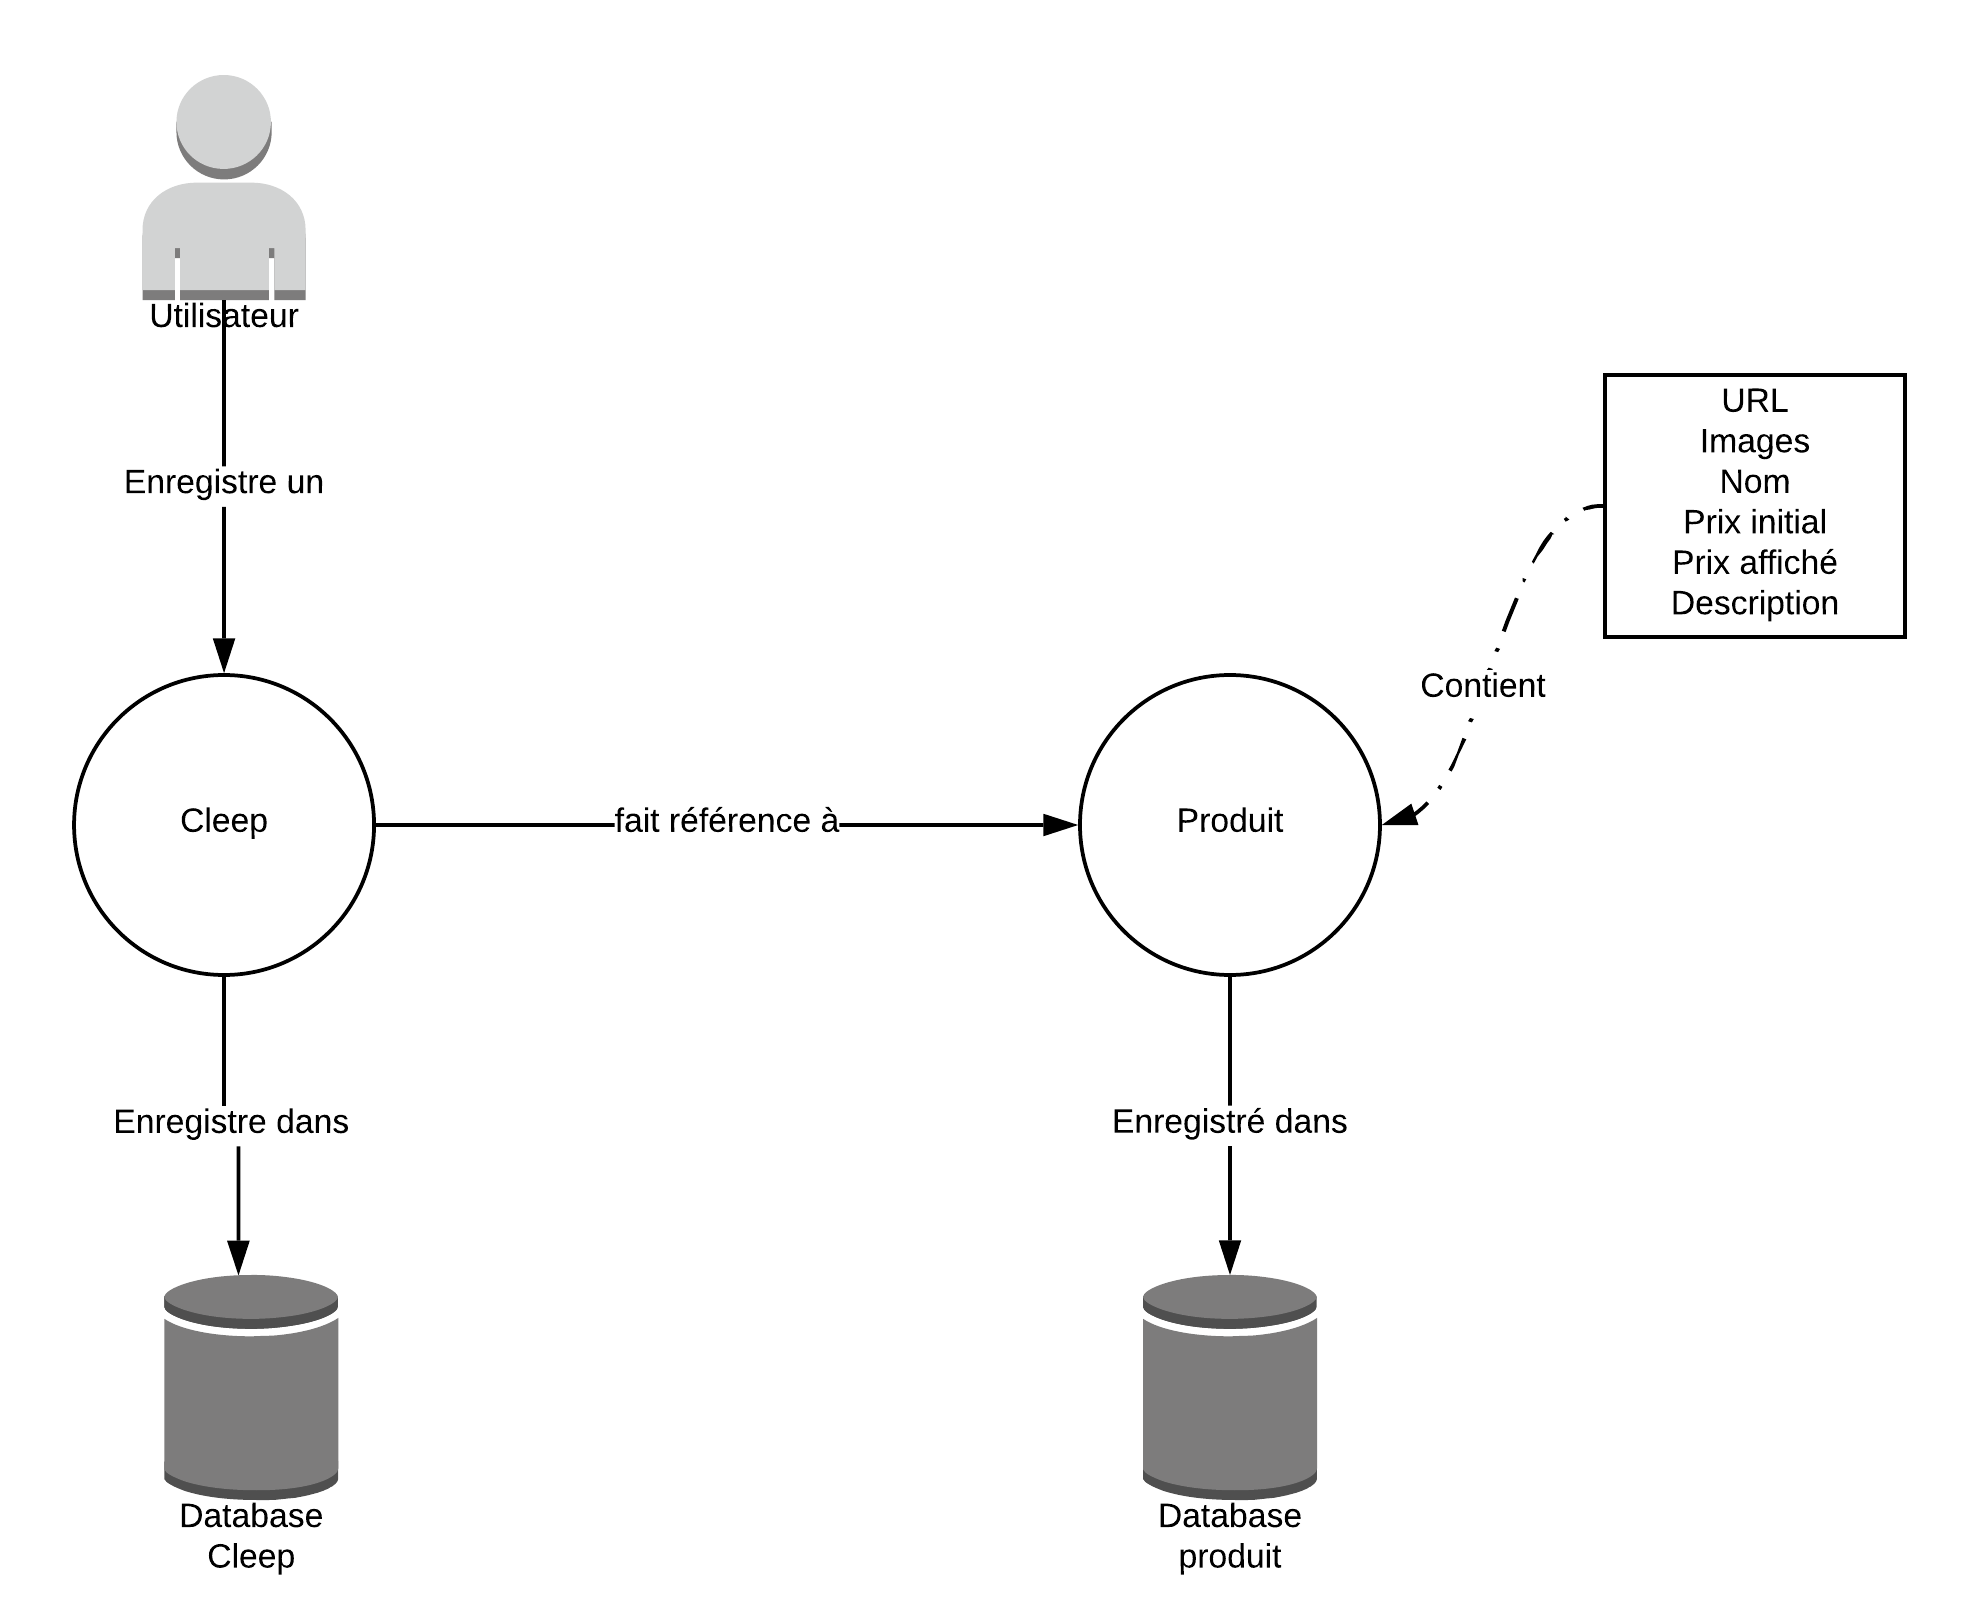
\includegraphics[keepaspectratio = true,scale=0.7]{scrapping.png}
	\caption{Organisation des données de cleep}
\end{figure}
\newpage

Relier un cleep à un produit est un défi pour l'application, car les utilisateurs sont plus enclins à rester dans l'environnement Cleep lorsqu'ils ont les informations à leur disposition dans l'application. En effet les cleeps contenant ces information, l'utilisateur est moins tenté de suivre le lien du produit et a plus de chance de rester sur l'application et parcourir les listes de clepp d'autres utilisateurs. \\
Cependant pour pouvoir faire cela, il faut récupérer les informations des produits au préalables. C'est ici qu'intervient le webscrapping. Les méta-données qui nous intéresse sont récupérées par ce moyen et entré dans la base de donnée. L'objectif de cette mission était donc d'enrichir la base de donnée des produits de manière automatique. 


\subsection{Travail effectué}
Cette sous-section relate le travail effectué sur cette mission.
\subsubsection{Contexte\\}
Avant mon arrivé, plusieurs methode de webscrapping étaient déjà utilisées:
\begin{itemize}
	\itemsep 0em
	\item Méthode automatique
	\item Méthode spécifique
\end{itemize}
\paragraph{Méthode automatique:\\}
Cette méthode était la plus utilisée pour récupérer les informations des produits. L'utilisateur rentre un lien dans l'application, par la suite ce lien est envoyé au serveur sur lequel la méthode est implémentée. Le serveur génère un navigateur internet sans interface graphique (headless browser) et requête le lien internet rentré par l'utilisateur. Ensuite, en analysant les balises du code HTML chargé, l'algorithme par certaines règles essaie de récupérer les méta-données. Ces informations sont alors transférés à l'utilisateur. Le schéma ci-après décrit le processus.
\begin{figure}[!h]
	\centering
	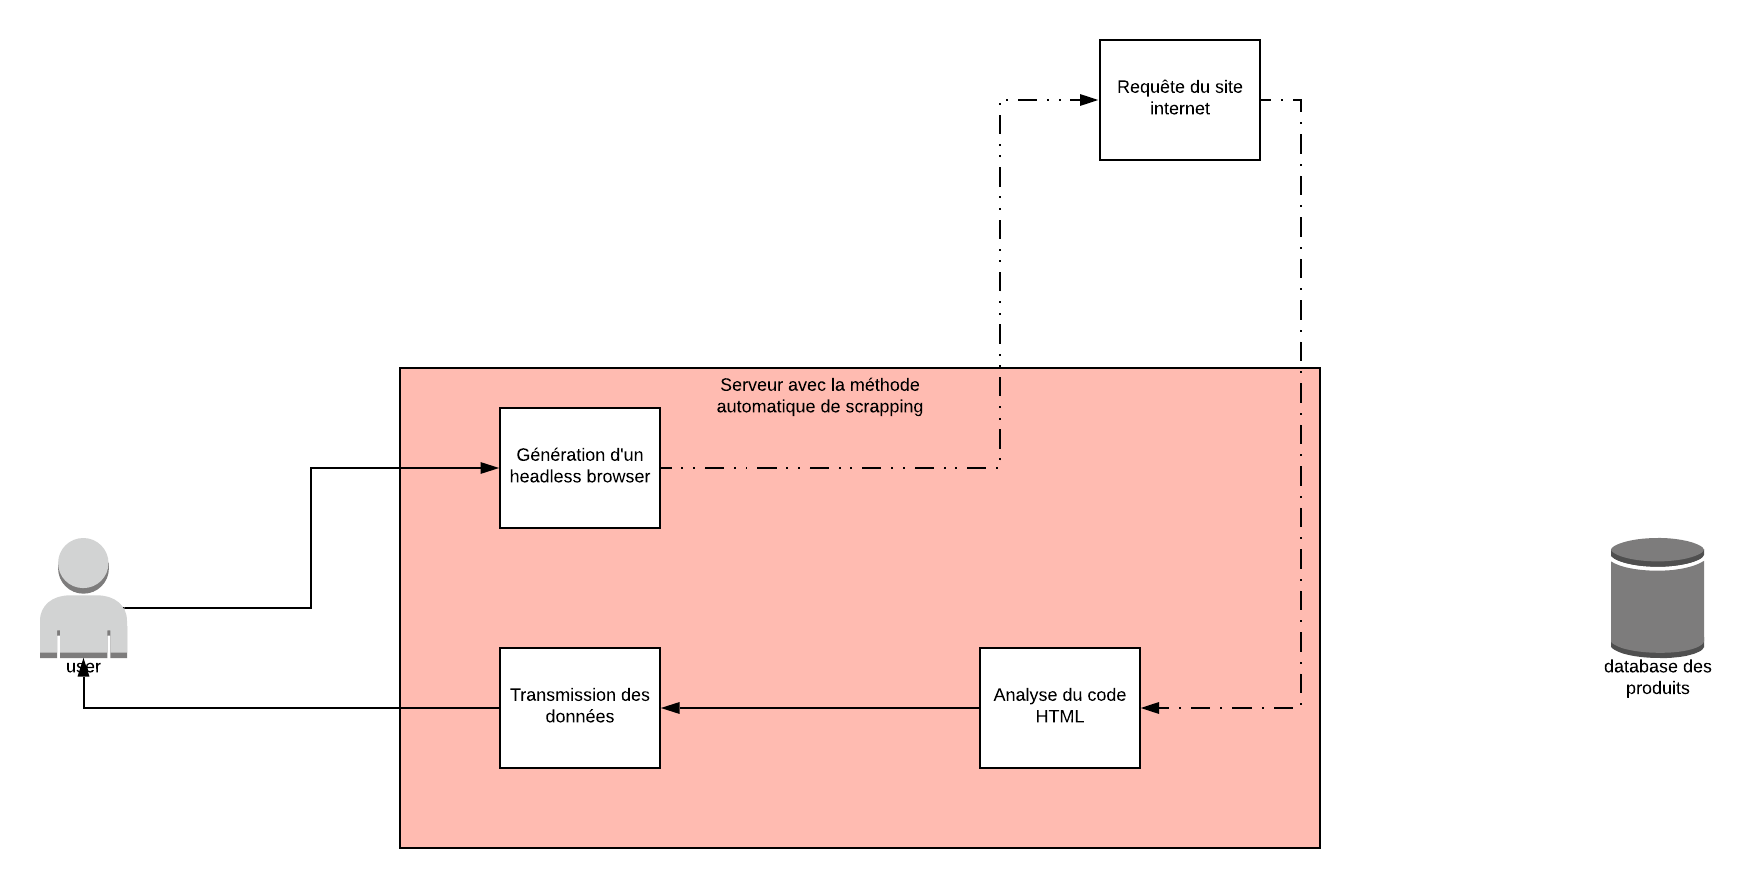
\includegraphics[keepaspectratio = true,scale=0.6]{browserInject.png}
	\caption{Méthode automatique}
\end{figure}
Bien que cette méthode de scrapping soit indépendant du site internet, elle reste néanmoins assez "précaire", car il est rare d'avoir toutes les informations nécessaires à disposition. Il est fréquent d'avoir certains attributs manquant, car les règles créées pour l'analyse du code HTML n'était pas assez vaste. Prenons les deux sites internet suivant :\\
\newpage
Site N°1:
\lstinputlisting[language=html]{site.html}

Site N°2:
\lstinputlisting[language=html]{site2.html}

Dans le cas N°1, il est facile de mettre une règle pour récupérer le prix dans le meta tag. Dans le cas N°2 cependant, le prix est "juste" inclut dans une balise <p>, rendant la règle précédente inutile. La méthode automatique implique donc beaucoup d'erreurs et d'approximations. Pour des soucis de mémoire, ces données ne sont pas enregistrées dans la base de donnée des produits, afin de ne pas garder les "fausse" données récupérées.
Cette méthode pose un autre soucis, c'est son temps de réponse. En effet, afin de scrapper le site, le serveur est obligé de générer un headless browser, de faire la requête, analyser le code HTML pour finalement retourner la réponse. Le temps de réponse doit être relativement bas, car l'utilisateur au moment du cleep doit pouvoir continuer ses activités sur Internet sans être interrompu trop longtemps par le temps que met Cleep à cleeper son produit, et donc eviter toute frustration.

\paragraph{Méthode spcéifique:\\}
C'est sur ce sujet que s'est concentré mon travail. Le principe de cette méthode est de prendre les sites internet un à un et d'appliquer un script de webscrapping qui leur est propre. Cela permet d'éviter les problèmes rencontrés précédemment.
La structure du code HTML derrière les pages produits est dans la quasi-totalité des cas la même pour un nom de domaine particulier. Il est possible que selon les sous-domaines d'un site cette page varie, par exemple pour la fnac on a:
\begin{itemize}
	\itemsep 0em
	\item https://livre.fnac.com/a13195869/Agnes-Martin-Lugand-A-la-lumiere-du-petit-matin
	\item https://jeux-video.fnac.com/a13608859/LEGEND-OF-ZELDA-LINKS-AWAKENING-FR-SWITCH-Jeu-Nintendo-Switch
	\item ...
\end{itemize}
Dans ce cas, on distingue les différents cas et ensuite on analyse le code HTML de chacune de ces pages. Cette méthode est bien plus fiable et donne de meilleurs résultats sur les méta-données requise.\\
Par ailleurs, afin de réduire le temps de réponse, une difficulté est rajouté : la génération d'un headless browser est supprimée m'obligeant à travailler avec le code source de la page (ie le résultat d'une requête cURL à la page), et les requêtes API.\\
En effet la génération d'un navigateur permettait de faciliter la tâche, car le code HTML étant totalement généré, il suffisait de récupérer le contenu des balises afin d'obtenir les informations nécessaires. Cependant via une requête cURL (ie le code source de la page), les script JavaScript ne sont pas déclenchés, il faut donc chercher au travers des differents script et requêtes API les éléments que l'on souhaite récupérer.

\begin{figure}[!h]
	\centering
	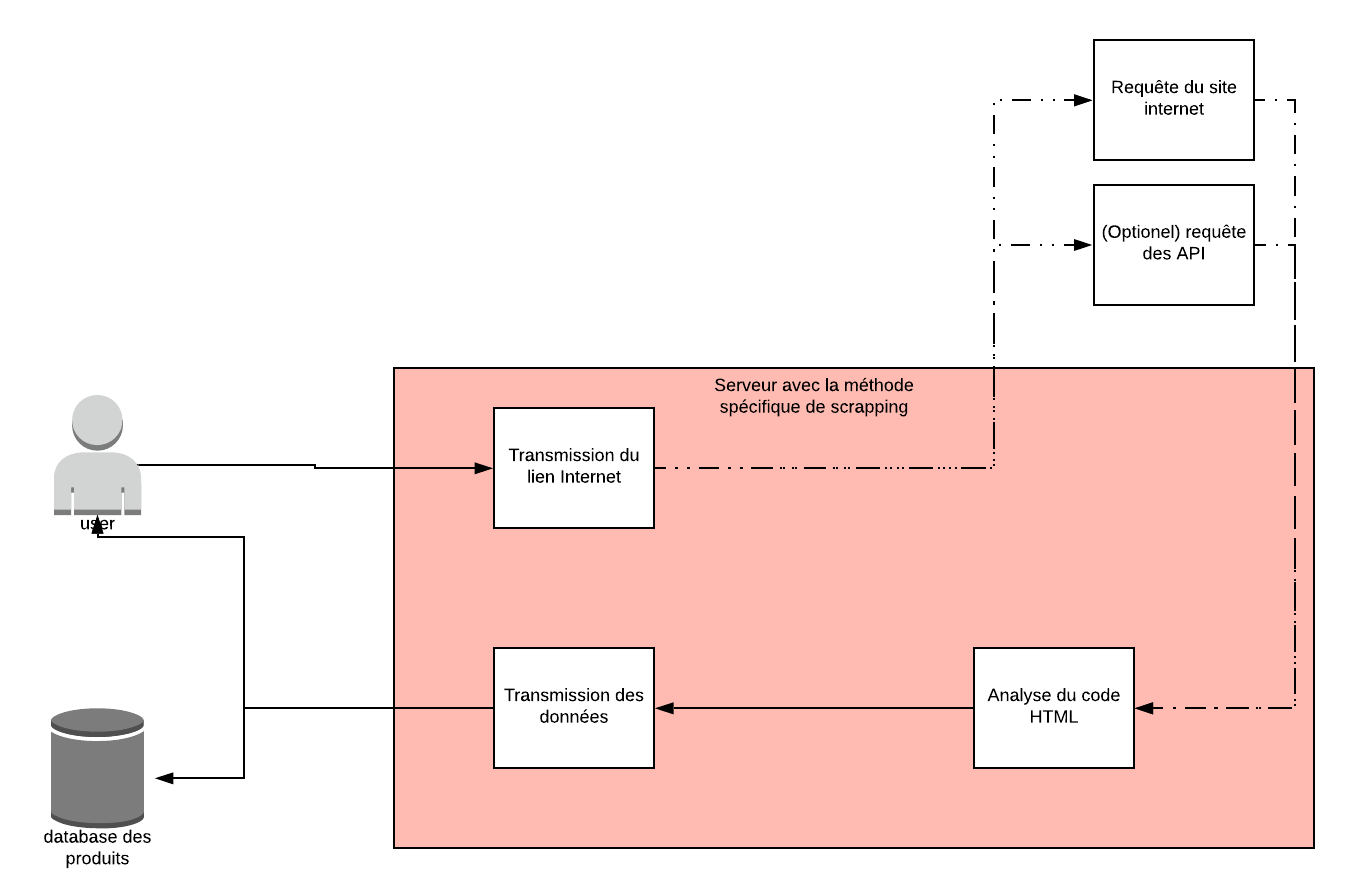
\includegraphics[keepaspectratio = true,scale=0.6]{specific.png}
	\caption{Méthode spécifique}
	\label{fig:methspec}
\end{figure}

\newpage

\paragraph{Démarche\\}
Le processus \textbf{figure \ref{fig:methspec}} montre les différentes étapes de la méthode spécifique. Mon travail s'est principalement concentré sur l'algorithme analysant un site web en particulier et la gestion des requêtes.\\
Prenons l'exemple suivant \cite{fnac} :
\begin{figure}[!h]
	\centering
	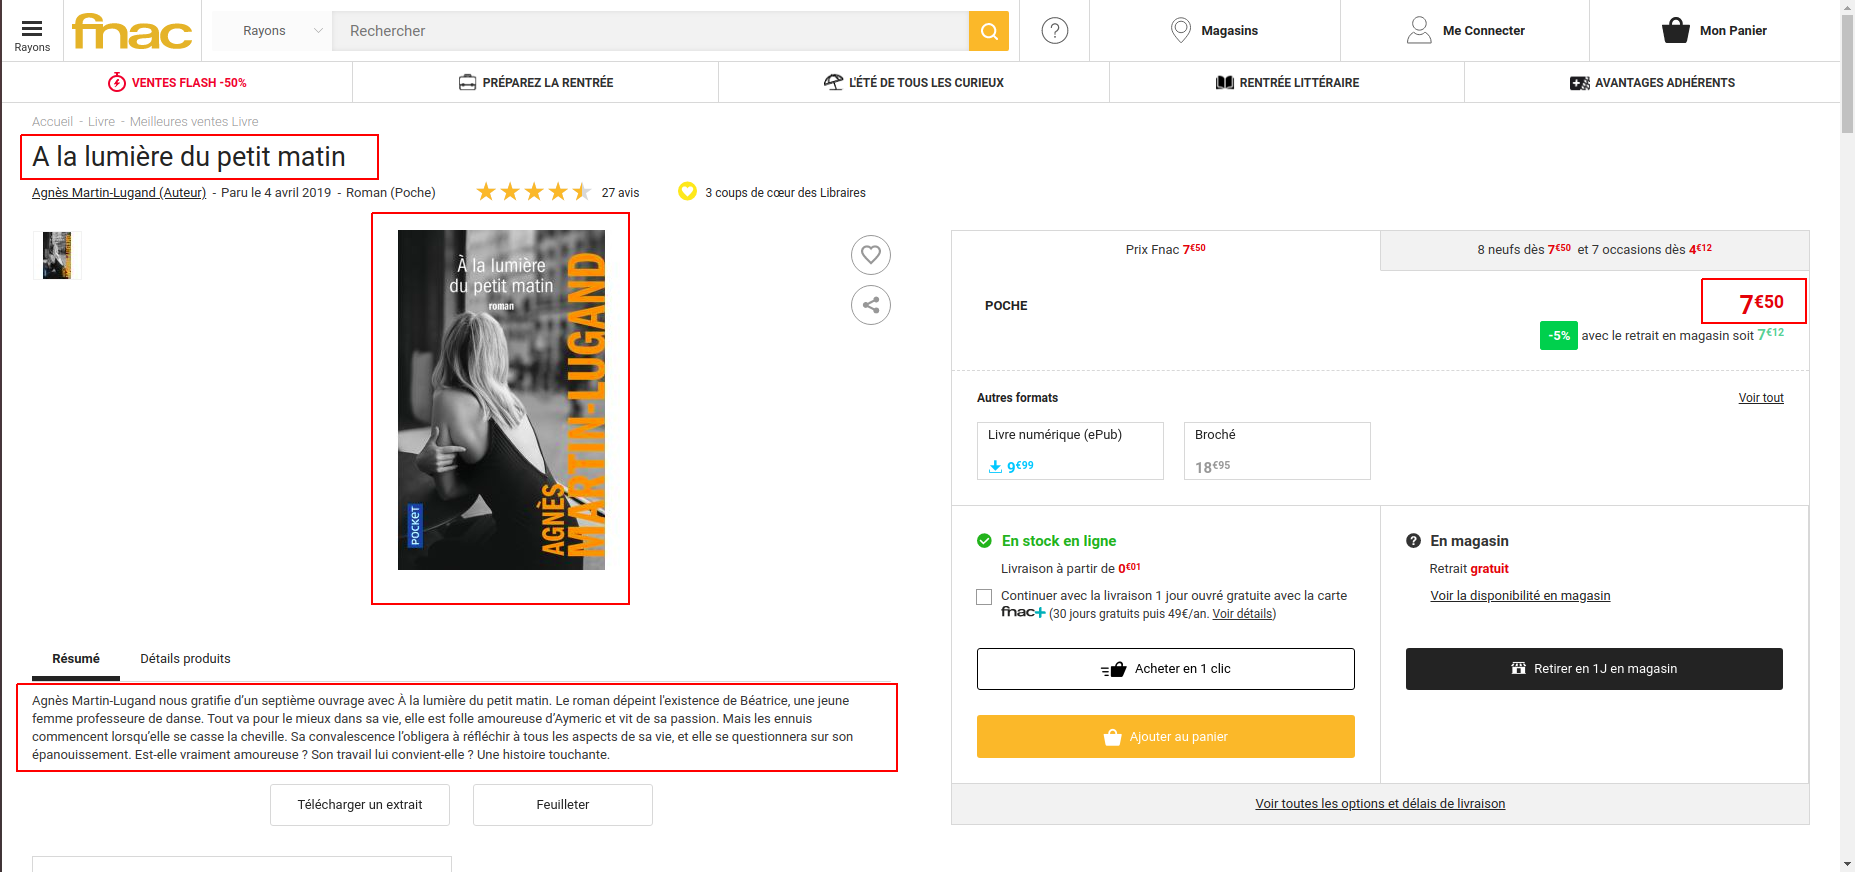
\includegraphics[keepaspectratio = true,scale=0.25]{fnac.png}
	\caption{Exemple fnac}
\end{figure}
Les encadrés rouges correspondent aux éléments que l'on doit récupérer. Vous pouvez retrouver en annexe une version allégé du code HTML (Annexe 9.1). Il est alors facile de comprendre que récupérer l'attribut $data-src-zoom$ de la balise <li> nous permet de récupérer l'image et le JSON quant à lui permet de récupérer les autres éléments requis.\\
La démarche adopter pour scrapper les différents sites à toujours été la même. Tout d'abord on analyse le code source afin de savoir quels éléments sont à récupérer. Ensuite on teste avec plusieurs liens différents afin de tester la robustesse de l'algorithme. Une validation finale était faite côté client, et ensuite l'algorithme était mis en production.\\ \\
Le dernier point nécessitant du travail : où trouver les liens permettant de scrapper les produits et peupler la base de donnée? L'ensemble des liens déjà cleepés sont enregistrés, et donc peuvent être utilisé pour répondre à cette question. Le client possédait déjà un script permettant de trier les liens par nom de domaines. Ainsi pour chaque nom de domaine que j'ai traité, j'ai du trié les liens pertinents (ie de produits) des liens inutiles (page principal, page de catégories etc). Par exemple, pour la fnac certains utilisateurs ont cleepé des pages présentant plusieurs produit \cite{mve} ce qui ne convient pas au processus détaillé auparavant.

\paragraph{Résultats\\}
A la fin de cette mission, j'ai développé un script de webscrapping pour plus de 56 sites différents. Cela a permis à Cleep de peupler sa base d'environ 220 000 produits différents.\\
Sur une vision plus large, les utilisateurs passent en moyenne plus de temps sur l'application (effet recherché), mais aussi ils ont tendance à cleeper plus de produit sur les sites dont le webscrapping a été fait.

\subsection{Vision critique et apport personnel}

La mission de webscrapping était plutôt simple, dans le sens qu'une fois les notions de webscrapping acquises, cette mission consistait à analyser un code HTML et les requêtes faits en javascript, pour trouver les informations nécessaires. Mon apport personnel s'est plus concentrés sur les discussions avec le client au sujet de l'amélioration du scrapper générique et le choix des technologies ainsi que la compréhension de l'infrastructure de Cleep.

\subsubsection{Scrapper générique\\}
Le scrapper générique déjà présent n'était pas assez efficaces pour pouvoir enregistrer les données des produits et il était trop lent pour être utilisé en production indéfiniment (pour l'instant, si un lien n'appartient pas à la liste des 56 domaines scrappés, il passe par le scrapper générique). Comme il n'est pas non plus possible de scrapper de manière spécifique l'ensemble des sites commerciaux existants (la base de donées de Cleep compte plus de 8000 nom de domaines différents), j'ai discuté avec le client sur la nécessité d'un scrapper générique plus performant.\\
Ainsi en parallèle, j'ai essayé de developper un scrapper générique plus performant n'utilisant pas un "headless browser". La valeur ajouté de Cleep reposant sur les images du produit enregistré dans l'application, j'ai travaillé sur un scrapper générique permettant de récupérer les images du produit.\\
Ce scrapper suit les 2 étapes suivantes :
\begin{itemize}
	\itemsep 0em
	\item Récupérations des liens "dynamique" de la page HTML
	\item Clustering des liens
\end{itemize}
\paragraph{Récupérations des liens "dynamique" de la page HTML:\\}
Cette étape consiste à récupérer l'ensemble des liens images de la page n'étant des liens statique. Un lien image est considéré comme statique s'il est présent plusieurs fois sur différentes pages. En générale ces images sont les logos et autre widgets communément présents. L'exemple \textbf{figure \ref{fig:stats}} ci-après montre les images statiques sur le site de la fnac. Une fois connus, ces liens ne sont pas pris en compte par le scrapper générique.\\ 
Ainsi, à la fin de l'étape 1 (cf \textbf{figure \ref{fig:step1}} pour voir le procédé), l'ensemble des liens dynamique (ie liens d'images changeantes) est connu. Cependant, parmis ces images nous avons les images du produits, mais aussi celle fournies par les recommandations. Il faut donc trouver un moyen de séparer ces images .

\begin{figure}[!h]
	\centering
	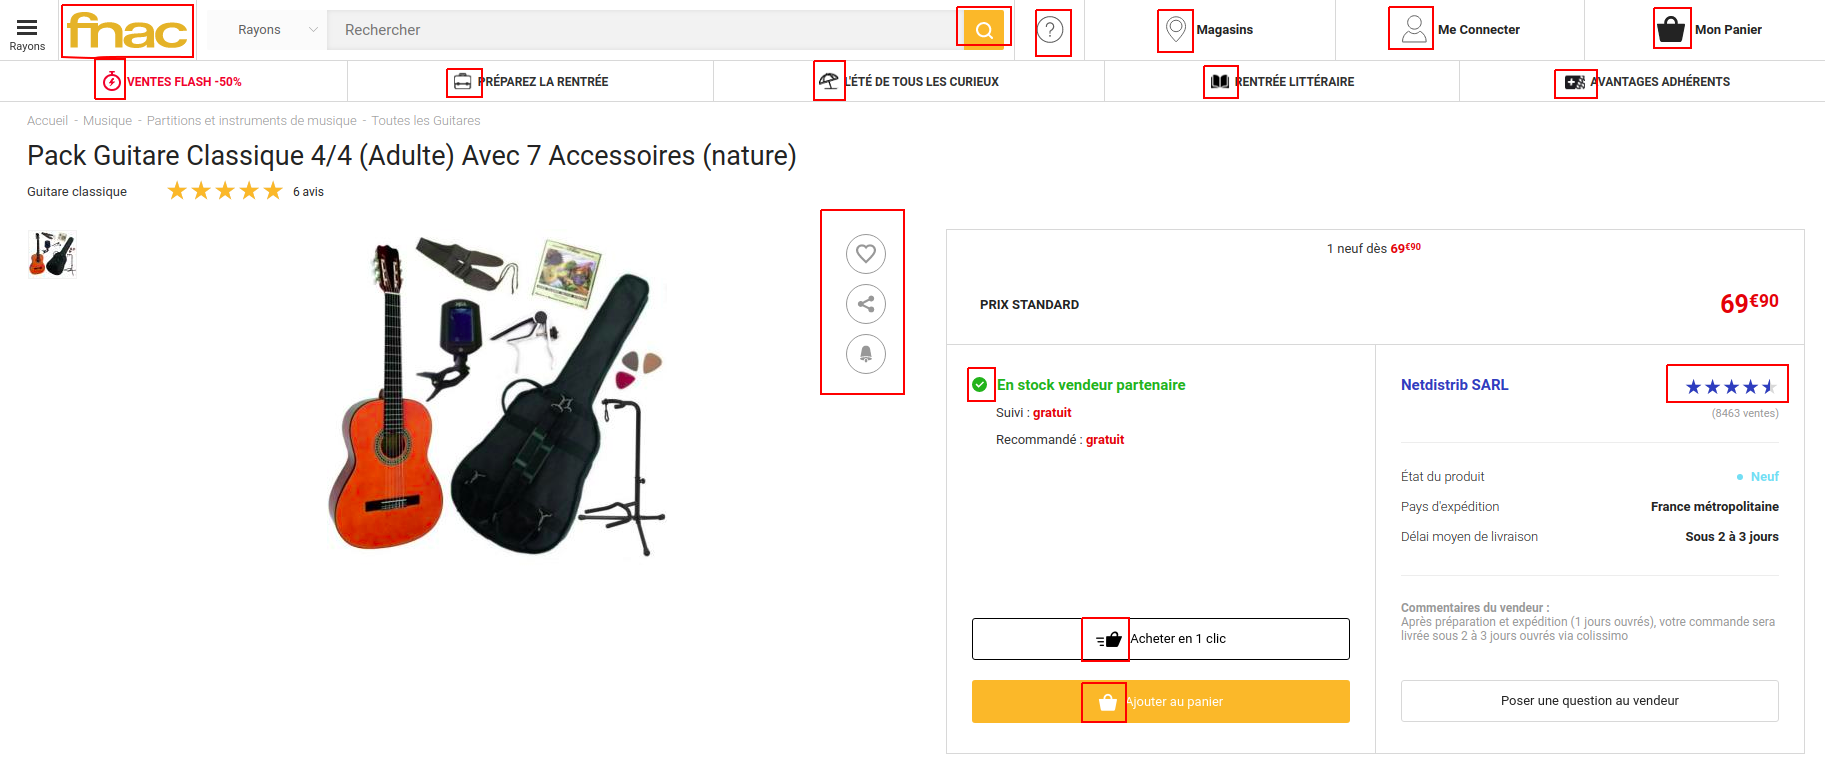
\includegraphics[keepaspectratio = true,scale=0.25]{static.png}
	\caption{Exemple d'images statiques}
	\label{fig:stats}
\end{figure}

 
\begin{figure}[!h]
	\centering
	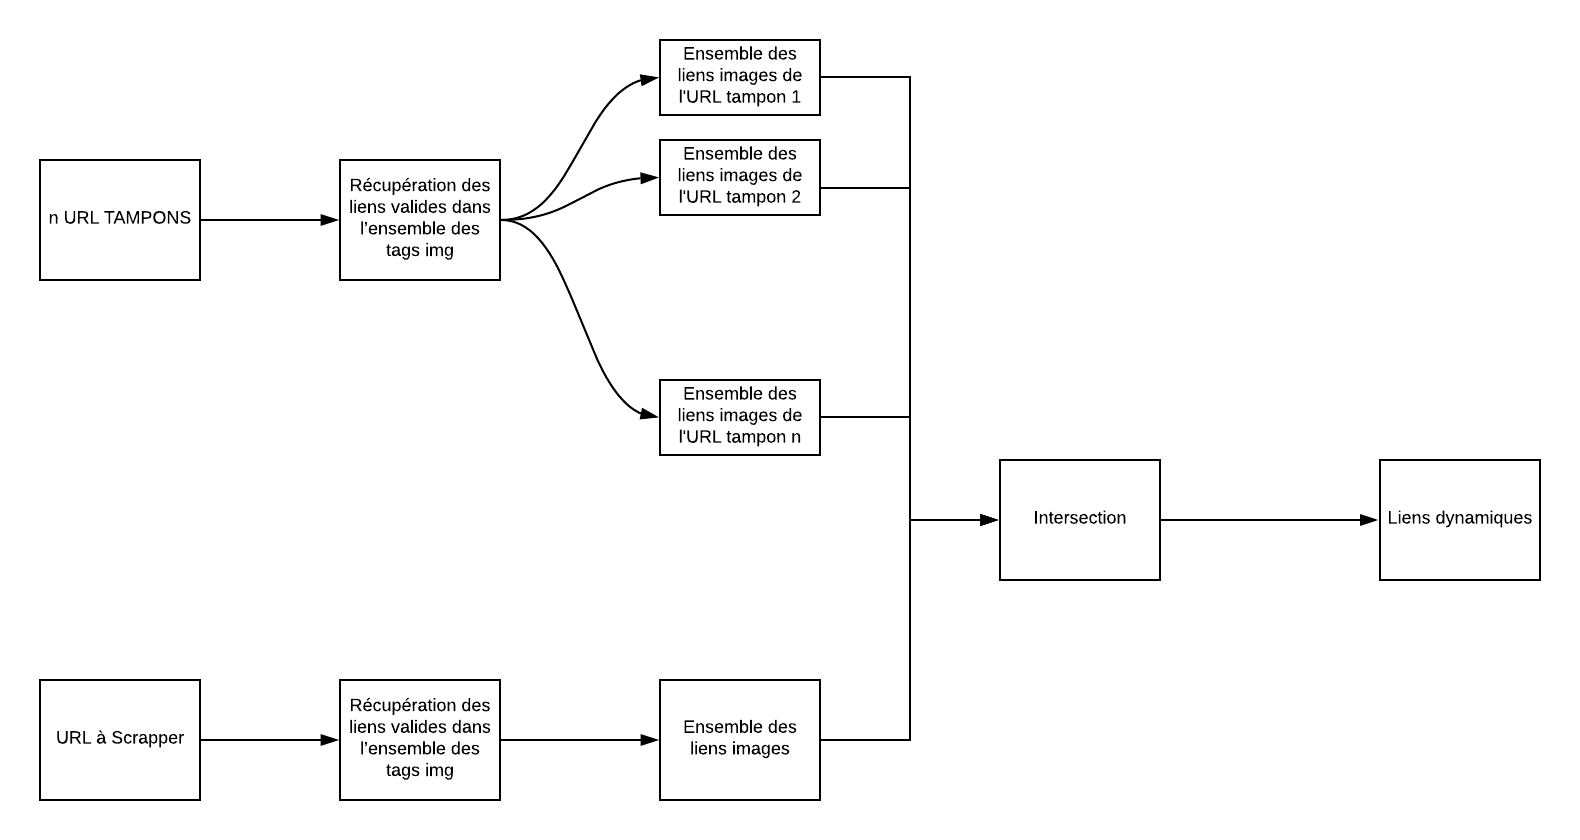
\includegraphics[keepaspectratio = true,scale=0.4]{step1.png}
	\caption{Etape 1}
	\label{fig:step1}
\end{figure}

\paragraph{Clustering des liens\\}
Le but ici est de regrouper les liens de recommandations entre eux et les liens concernant le produits entre eux aussi. Pour cela j'ai utilisé un algorithme de clustering : dbscan. Le clustering se fait sur la distance en nombre de caractère dans le code HTML par rapport au début du code.\\
Cela permet donc d'avoir en général 2 cluster distincts. En me basant sur l'ensemble des sites que j'ai scrappé auparavant, le 1er cluster est choisi comme celui contenant les images que l'on souhaite. Ainsi à la fin de cette étape on est sensé avoir l'ensemble des images du produit. Afin de vérifier si les liens sont bien ceux recherchés, on compare les liens entre eux en utilisant la distance de Levenshtein \cite{levenshtein}. La distance de Levenshtein entre deux chaînes de caractère $A$ et $B$ est le nombre minimum de transformation (ajout/suppression/changement d'un caractère) pour passer de $A$ à $B$. Ainsi, si dans le cluster, un lien paraît plus éloigné des autres, il est retiré de la liste.\\
Cette règle se base sur le fait que les images d'un même produits ont souvent des liens très similaires et sont différencié par un identifiant dans l'URL. 

\paragraph{Tests et résultats\\}
Les tests ont été réalisé sur une vingtaine de site que j'avais au préalable scrapper afin de pouvoir évaluer la différence. Il apparaît que ce scrapper générique arrive à récupérer toutes les images d'un produit spécifique. Cependant, il récupère trop d'image dans le sens où il peut récupérer 4 fois la même image mais ayant des tailles différentes. Encore une fois, pour des raisons de capacités mémoire, cette solution n'a pas été retenue par le client en l'état, mais est toujours en cours de développement.


\subsubsection{Technologie utilisée\\}
L'ensemble du travail a été réalisé en NodeJS (interpreteur Javascript). Cette technologie a été utilisé car l'ensemble de l'architecture client était en NodeJS. Il était possible de travailler avec les librairies Python permettant de scrapper et faire des requetes HTML (scrappy, beautifulsoup) car cette partie est plutôt indépendante. Cependant pour éviter l'overhead introduit par un changement de langage, j'ai préféré suivre le langage du client.\\
Par ailleurs, plusieurs sites internet ont des protections vis à vis du webscrapping. En effet les requêtes fait aux différents serveurs affecte les capacités de ces derniers. Ainsi deux problèmes se sont posés:
\begin{itemize}
	\itemsep 0em
	\item Ne pas lancer "involontairement" une attaque contre les serveur du site en question: pour cela on a trouvé une certaine limite temporelle avec le client
	\item Les adresses IP des serveurs de Cleep qui étaient déjà sur liste noire de plusieurs sites.
\end{itemize}

Le deuxième problème s'explique par une technologie de protection employé par les site internet contre le webscrapping : Datadome. Datadome detecte si une requête est faite par un utilisateur ou un robot en regardant si le javascript de la page est chargé et executé. Si ce dernier n'est pas executé, il s'agit probablement d'un bot ayant requêté uniquement le code source de la page, ce qui est exactement notre cas. Une fois detecté par Datadome, l'adresse IP qui a servi pour la requête est mise sur liste noire et il n'est plus possible de faire de requête.\\

La solution trouvé avec le client est de passer par un service de Proxy payant : Luminati, qui permet de changer d'adresse IP à chaque requête et donc de pouvoir utiliser les scripts de scrapping. Il est a noté que ce service facture à la requête, ainsi seul les sites ayant une protections datadome ou similaire passent par ce proxy.

\newpage

\section{Mission : Moteur de recommandation pour Cleep (2.5 mois)}

Cette partie est consacrée au développement d'un moteur de recommandation pour la start-up Cleep. Cette mission fait directement suite à celle de webscrapping et reste dans l'esprit de développer des fonctions nécessaires à la croissance de l'application. Lors de cette mission, j'ai profité d'une grande autonomie car aucune solutions antérieures n'existaient auparavant. J'étais cependant en contact avec Damien Meurisse, co-fondateur de Cleep, et Paul Saffers, consultant datascientist à Sia Partners, afin de critiquer et valider mon avancement 

\subsection{Contexte et problématique}

Le but de cette mission est de développer un moteur de recommandation : à partir d'un élément et des données qui lui sont liées, le moteur doit retourner un ou plusieurs éléments similaires. Cette pratique est vastement répandue parmi les sites marchands/ sites de services (Amazon, Netflix, Pinterest ...).\\

Avant le début de cette mission, Cleep n'avait pas de moteur de recommandation à proprement dit, certaines ébauches de moteur avait été faites, mais rien de concret. Pour une application comme Cleep dont le principe est de rendre l'utilisateur indépendant des sites marchands et de lui offrir une alternative au shopping basique sur Internet, la création d'un moteur de recommandation devenait nécessaire.\\
En effet, il est possible de partager au travers de l'application les produits cleepés ainsi que les listes de cleeps. Un utilisateur peut donc voir les cleeps d'autres utilisateurs et en particulier ceux correspondants à ses centres d'intérêts. Les interactions avec les cleeps déjà disponibles sur la plateforme sont donc importantes, plus un utilisateur navigue sur Cleep, plus il passe de temps sur l'application ce qui le fidélise. Cependant sans moteur de recommandation, la navigation et la découverte de nouveaux cleeps est assez difficile pour l'utilisateur. Celle-ci passe soit par la bar de recherche pour la recherche de cleep(s) spécifique(s), soit par les pages catégories (triant les cleeps des utilisateurs par catégorie).\\
C'est donc dans l'optique de créer un moteur de recommandation fonctionnel et adapté à l'architecture déjà présente de Cleep que la mission m'a été confiée.

\paragraph{Objectif(s)\\}

L'objectif premier de cette mission qui a durée 2.5 mois était de créer un moteur de recommandation à partir des données de Cleep. Cette mission s'est divisée en deux grandes étapes:
\begin{itemize}
	\itemsep 0em
	\item Etudes des différents moteur de recommandations existant et études des bases de données en graphe
	\item Implémentation sur la technologie choisie d'un moteur de recommandation pour Cleep
\end{itemize}
La deuxième étape inclue l'ensemble des discussions avec le client au sujet des caractéristiques du moteur de recommandation, comment il est sensé se comporter, les améliorations possibles par rapport au cas de Cleep, ainsi que les manières de tester et valider la solution apportée.\\
Dans le cas précis de Cleep, un moteur de recommandation consiste à fournir à partir d'un cleep un certains nombre de cleep pouvant être utile à l'utilisateur (cf schéma \textbf{figure \ref{fig:reco}}). 

\begin{figure}[!h]
	\centering
	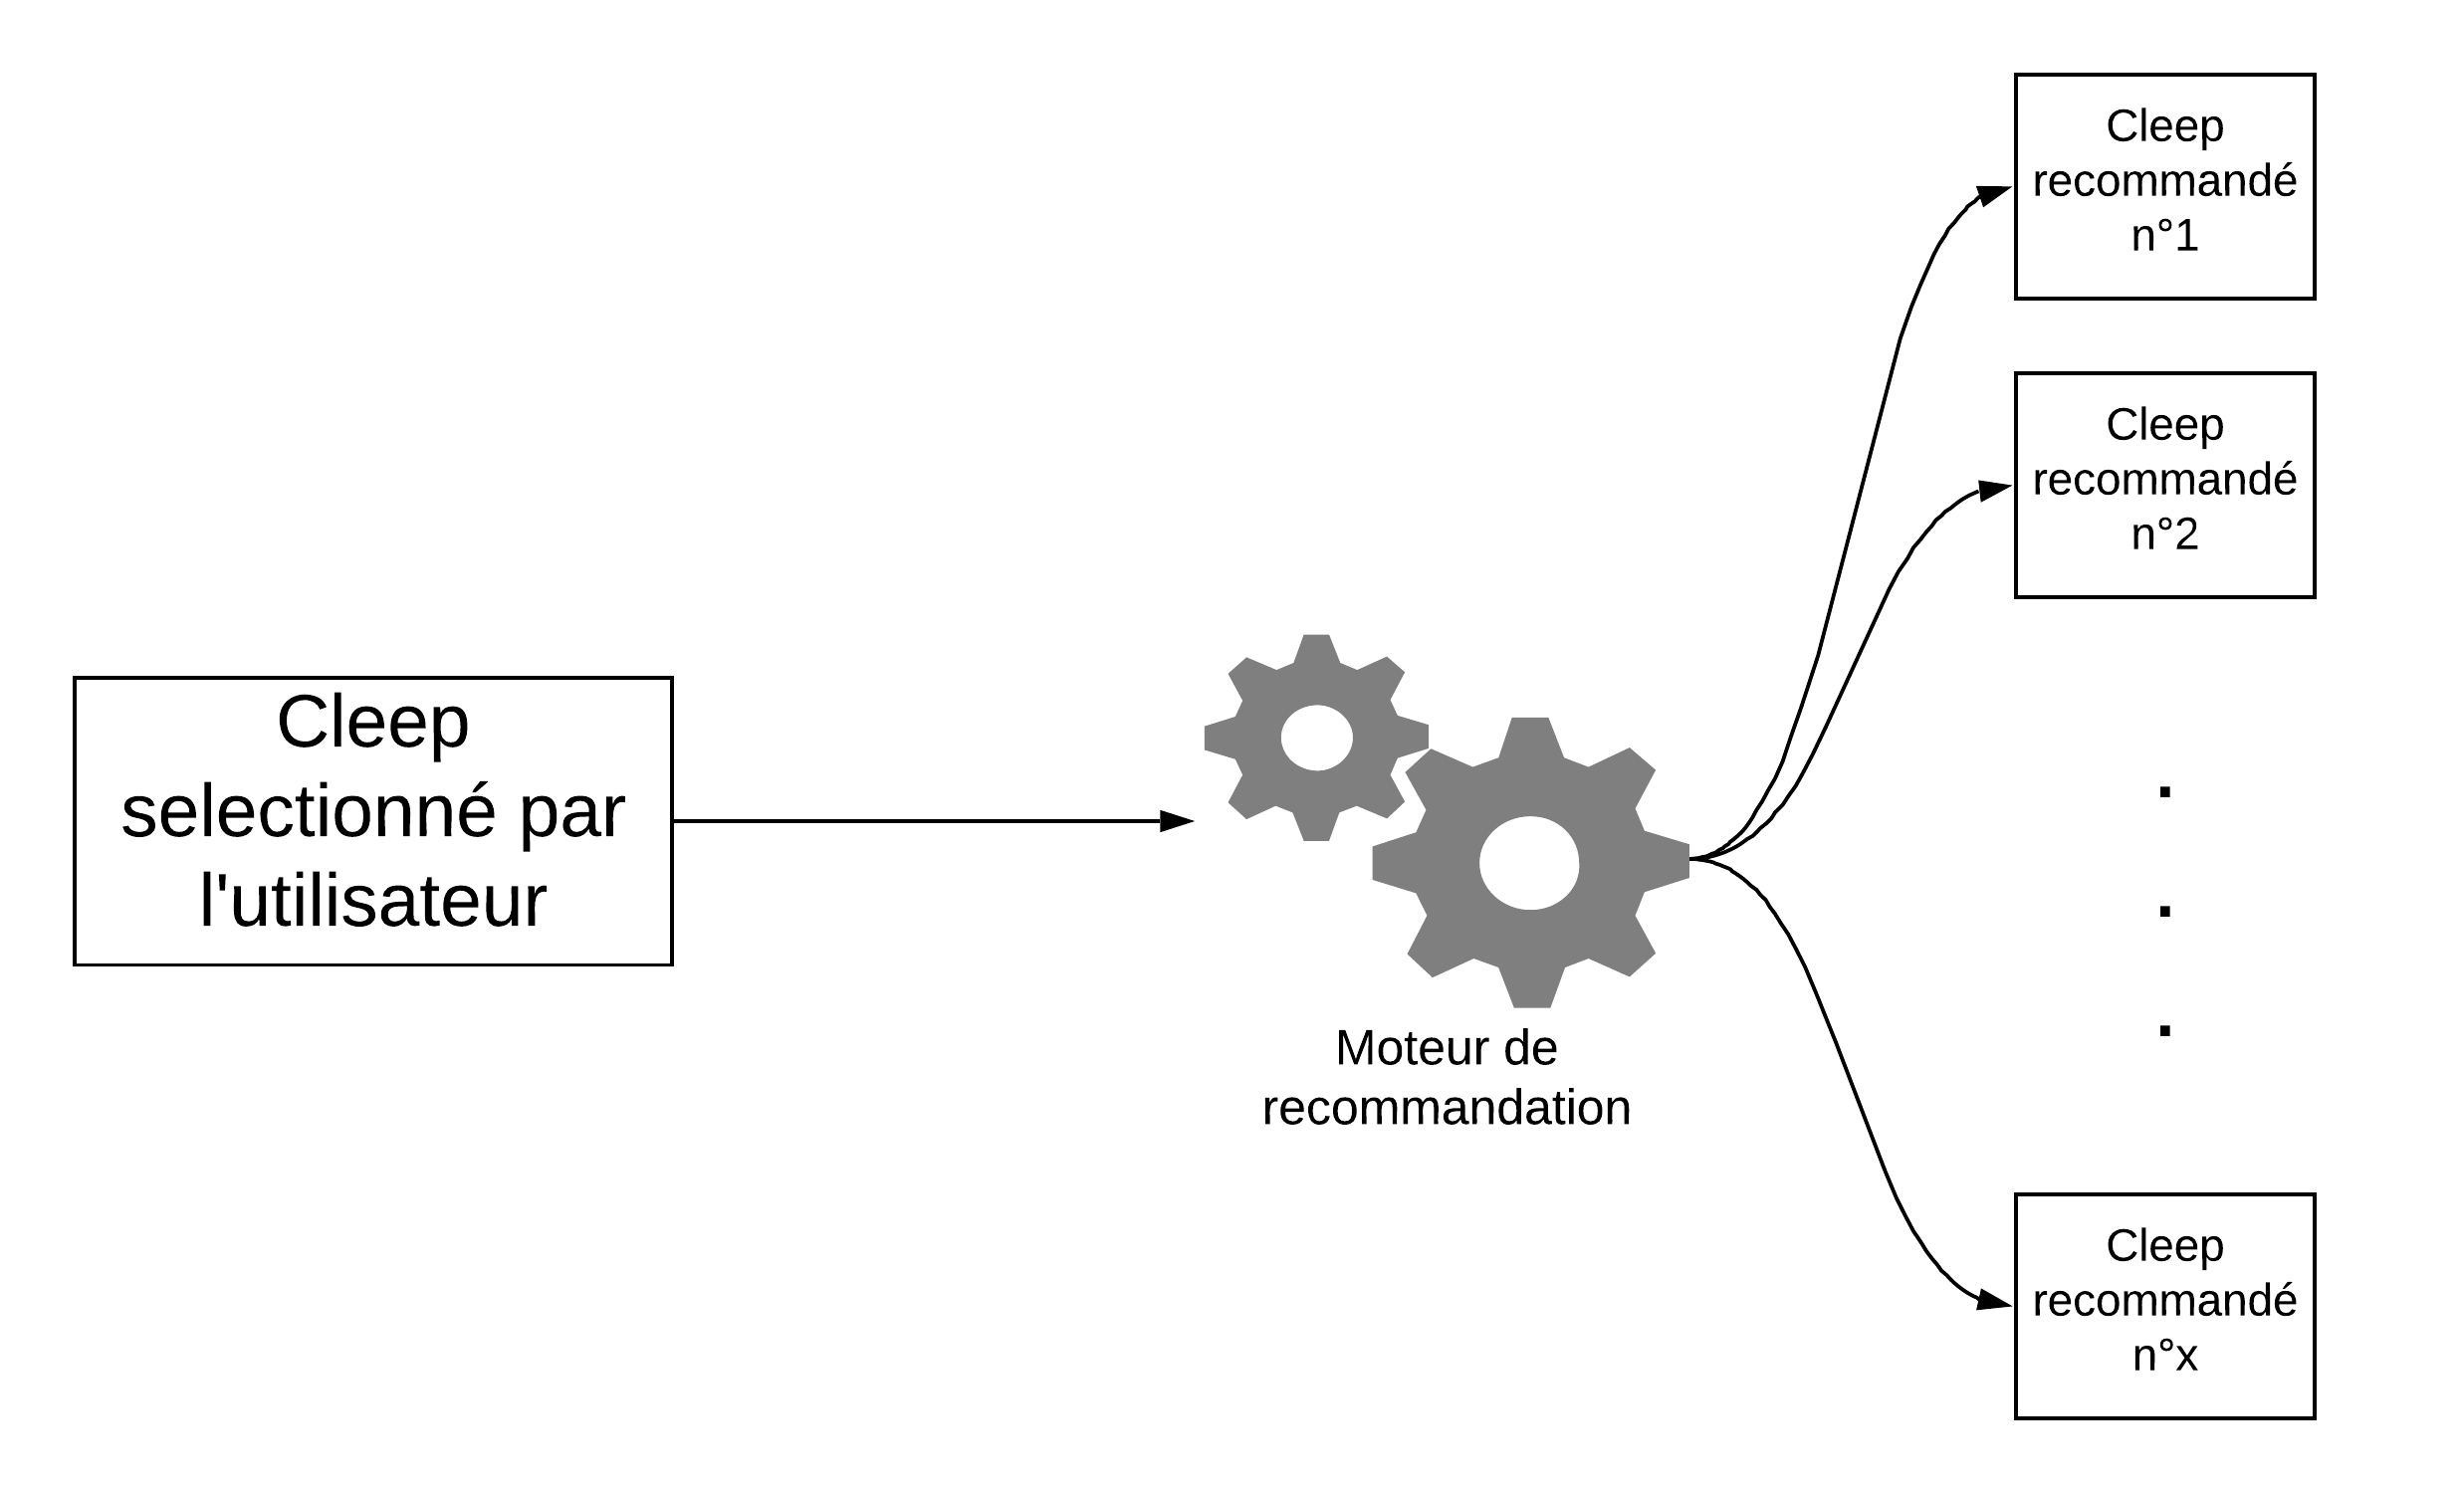
\includegraphics[keepaspectratio = true,scale=0.4]{reco.png}
	\caption{Etape 1}
	\label{fig:reco}
\end{figure}

La boite noire qu'est pour l'instant le moteur de recommandation reposera sur l'ensemble des éléments présents dans la base de donnée de Cleep afin d'avoir des recommandations précises et pertinentes. En effet, plus l'analyse des données et de leurs relations est poussée, plus le moteur retournera des cleeps pertinents. Tout du moins pertinent par rapport aux tendances évoquées par les données.

\paragraph{État initial}
Avant le début de ma mission, il y avait déjà eu quelques idée pour la création et le développement d'un moteur de recommandation.\\
Cleep est une application qui repose beaucoup sur le visuel, et donc sur les images des produits. Cette image permet à l'utilisateur de reconnaître la nature du produit et donc de savoir ce qu'il a cleepé. Ainsi une idée envisagée était de baser le moteur de recommandation uniquement sur l'analyse des images. Pour cela il existe une API developpé par Google qui permet de fournir des "tags images" ainsi qu'une pourcentage de confiance associé. Dans la \textbf{figure \ref{fig:ggviz}}, on peut voir l'application de l'algorithme derrière cette API sur un pull.\\

\begin{figure}[!h]
	\centering
	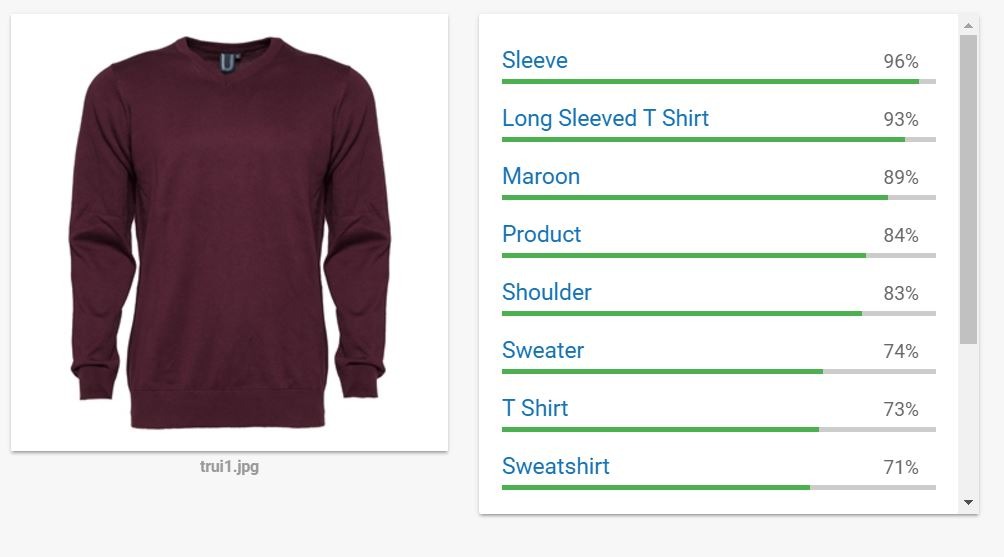
\includegraphics[keepaspectratio = true,scale=0.4]{ggvision.jpg}
	\caption{Etape 1}
	\label{fig:ggviz}
\end{figure}

Dans cette ébauche de moteur de recommandation, l'idée était donc de tagger toutes les images de la base de donnée en premier lieu. Ensuite, pour un cleep dont on veut les recommandations, on fait passer ses images par le même algorithme, et on récupère ses tags. La dernière étape du processus envisagé est de retourner les images ayant le plus de tags en commun avec ceux du cleep original, tout en prenant en compte le pourcentage de confiance.\\
Cette idée, bien que fonctionnelle, ne prend en compte qu'une infime partie de la base de donnée de Cleep (ie les images). Ainsi, il est très peu personnalisé et retourne des recommandations génériques. Le but premier de cette mission est donc d'utiliser au mieux l'ensemble des informations afin de fournir des recommandations personnalisées.

\paragraph{Écosystème de Cleep\\}
Il est nécessaire pour comprendre le travail que j'ai effectué de connaître l'ensemble des éléments à disposition dans la base de donnée Cleep. Je reviendrais plus en profondeur par la suite, en détaillant précisément le type de base ainsi que la structure choisie pour faire fonctionner ce moteur de recommandation.\\
\newpage

La base de donnée est composé de:
\begin{itemize}
	\item Informations de l'utilisateur anonymisées : son âge, son sexe, ses interêts ses interactions avec les sites internet marchands etc.
	\item Informations sur les cleeps : la liste à laquelle il est associé, ses tags provenant de google vision, sa date de créations, l'utilisateur qui l'a créé, et son statut (s'il est toujours en ligne ou s'il a été supprimé par son propriétaire)
	\item Information sur les listes de cleeps: son statut, son propriétaire et l'ensemble des personnes ayant accédé/partagé cette liste
\end{itemize}
Par ailleurs, les activités des utilisateurs sont enregistrées, ce qui donne des informations en plus, notamment sur les interactions entre les trois entités : cleeps, utilisateurs, listes. Sont a disposition les activités sur les relations suivantes:
\begin{figure}[!h]
	\centering
	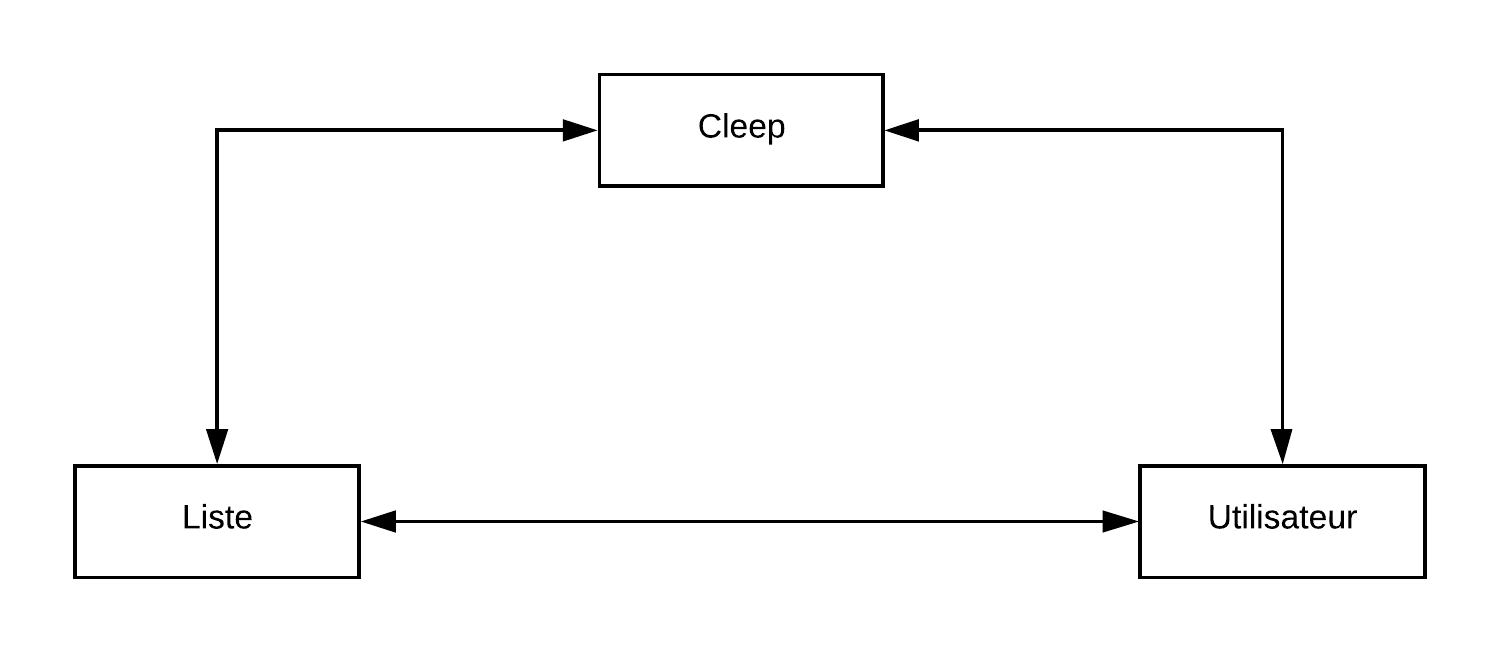
\includegraphics[keepaspectratio = true,scale=1]{relations.png}
	\caption{Etape 1}
	\label{fig:rel}
\end{figure}



\subsection{Travail effectué}
Dans cette partie je vais décrire le travail effecuté pour la création du moteur de recommandation et revenir sur les principales étapes de ce processus. Comme dit précédemment, cette mission s'est d'abord axée sur l'étude des système de recommandations déjà existant ainsi que les technologies qui leurs sont associées. Ensuite, il a fallu designer et implémenter le moteur de recommandation en se basant sur les conclusions de la première partie. 

\subsubsection{Étude des moteur de recommandations similaires}

Le cas de Cleep n'est pas du tout unique, il y a plusieurs exemples d'application similaires sur le marchés utilisant des moteurs de recommandations. On peut penser notamment à l'ensemble des sites marchands que j'ai scrappés en première partie. Chacun d'entre eux possède un système leur permettant de recommander des produits à partir d'un article.\\
Il y a donc autant de manière de faire un système de recommandation qu'il y a de site en proposant. Cependant il y a des objectifs clairs vis à vis de ce dernier :
\begin{itemize}
	\itemsep 0em
	\item A partir d'un articles, plusieurs articles doivent en ressortir
	\item La recommandations doit être personnalisée
	\item La recommandation doit être rapide
	\item La mise en place du système ne doit pas être chère
\end{itemize}
C'est donc avec ces objectifs que j'ai commencé les recherches.

\subsubsection{Article de recherche : moteur de recommandation de Pinterest\\}
Après quelques recherches, ma culture personnelle  ainsi que sur les conseils de Damien et Paul j'ai orienté mes recherches sur les moteurs de recommandations ayant une solution basé sur le parcours de graphe. Damien m'a alors recommandé la lecture de l'article de recherche sur le moteur de recommandation de Pinterest : Pixie \cite{pixie}.\\
Pinterest \cite{Pinterest}, est un réseau social, dont le principe est de partager de l'information via des photos, vidéos, GIFs. Chaque élément partagé peut avoir une description un titre et des tags au choix de l'utilisateur. Ce réseau est en général utilisé pour partager autour de certains centres d'intérêts comme par exemple la photographie, le sport, la cuisine etc. Le moteur de recommandation de Pinterest est donc une bonne source d'inspiration pour Cleep. Le parallèle se faisant sur le côté très graphique de l'application. Ce sont les images qui attirent l'œil avant tout, mais aussi sur le but du moteur qui est d'identifier les pins (entité regroupant l'ensemble des informations liés aux images sur Pinterest)/cleeps répondant au mieux à l'envie de l'utilisateur. Ainsi, pour les deux application ce n'est pas nécessairement de pousser à l'achat, mais de faire rester sur l'application qui est important.\\

Pixie est un moteur de recommandation basé sur le parcours d'un graphe en marche aléatoire. Le graphe créé pour Pixie se base sur l'ensemble des entités présentes dans l'écosystème Pinterest. Pour résumer, les noeuds du graphe sont les pins et les utilisateurs. Les arrêtes sont les relations : pins $\leftrightarrow$ pins, pins $\leftrightarrow$ utilisateurs, utilisateurs $\leftrightarrow$ pins. Chacune des entités (arrêtes et nœuds) contiennent de l'information.\\
Le graphe établit, il est alors possible d'établir une distance entre les pins. Cette distance est très importante car c'est elle qui va déterminer la qualité du moteur de recommandation. Le calcul de cette distance est spécifique à Pinterest, je ne vais donc pas la décrire. Cependant il est à noter que Pinterest utilise la quasi-totalité de l'information qu'il possède afin de calculer cette distance.\\
Il est possible de penser que le travail est fait et qu'il suffit uniquement de récupérer pour un pin les pins les plus proche de ce dernier sur le graphe. Cependant, comme le titre du papier de recherche l'indique, il y a plus de 3 milliards de pins et plus de 200 millions d'utilisateurs. Ainsi, pour chaque nœud il faudrait calculer la distance avec l'ensemble des autres nœuds, ce qui est très long voir impossible. Mais aussi il faudrait stocker cette donnée ce qui est aussi compliqué vu la taille des données. En effet, en supposant que le résultat soit un entier codé sur un 4 octets mais aussi que la distance pour aller d'un pin A à un pin B soit indépendant du chemin, il faudrait pour un nœud 12 gigaoctets. Soit pour l'ensemble de la base de donnée 36 exaoctets ($36.10^9$ $Go$). De plus, à chaque ajout de nœuds, il faudrait tout recalculer, car les relations peuvent changer.\\
Les problèmes de stockage, de calculs mais aussi de mise à jour en temps réel rendent la solution évoquée précédemment irréalisable. De plus vu que les arrêtes du graphe portent de l'information, la distance dépend bien du chemin parcouru ainsi les calculs ont été (volontairement) vu à la baisse.\\

Le papier répond à ces problèmes avec l'heuristique suivante :
\begin{itemize}
	\itemsep 0em
	\item Étape 1 : Récolte des informations sur le premier Pin
	\item Étape 2 : N marches aléatoires sur le graphe ($N \in \mathbb{N}$ )
	\item Étape 3 : Calcul du score (distance) pour chaque marche aléatoire avec le dernier pin disponible sur la marche.
	\item Étape 4 : Parmis les N scores, seul les pins recommandés ayant un socre supérieur à un seuil déterminé au préalable sont gardés
	\item Étape 5 : S'il n'y a pas assez de pins pour la recommandation, le processus est relancé 
	\item Étape 6 : Les recommandations sont poussées sur l'application et montrées à l'utilisateur
\end{itemize}
A partir de maintenant, le terme score désigne la distance calculé avec les informations et le terme distance la distance nœuds à nœuds.\\
Cette heuristique permet donc d'outrepasser l'ensemble des problèmes liés à la mémoire car les scores ne sont jamais sauvegardées. De plus le calcul du score dépend bien du chemin parcouru : il est possible d'avoir la situation où le même pin est retourné deux fois, sans pour autant avoir le même score car la traversée du graphe était différente. Comme c'est une heuristique, le résultat fournit n'est bien évidement pas la solution optimale, mais elle s'en rapproche pour un temps réalisable.\\
La critique qui peut être émise vis à vis cette heuristique est le côté marche aléatoire. Il va être fréquent de tomber sur les mêmes nœuds / les nœuds les plus proches (en terme de distance nœuds à nœuds). Au vu du nombre de noeuds existant dans la base de Pinterest (et existant aussi dans la base de Cleep), il est assez rare de tomber plusieurs fois sur le même chemin. Ensuite pour la deuxième critique, c'est le but même de l'heuristique, rester assez proche du nœud original. Plus on va loin dans la propagation dans le graphe, plus le nœud original est le voisin d'un voisin d'un voisin ... du nœud actuel. Il y a donc de base peu de relations entre les deux nœuds ce qui va en général retourner un mauvais score.\\

C'est à partir de cette heuristique que j'ai alors implémenté le moteur de recommandation pour Cleep. Cependant, je ne pouvais pas suivre l'ensemble de papier de Pinterest car il y avait quelques limitations en matière de ressources exigées.\\
Pinterest crée son graphe avec une partie de sa base de donnée. Ce sont les pins étant les plus tendances, et les plus vues pendant une période donnée qui y sont inclus, mais aussi les utilisateurs ayant le plus d'interactions avec les autres/ les pins. Le graphe est créé en C++ de manière dynamique. Ainsi le graphe est stocké en mémoire RAM des serveurs, l'heuristique lui est ensuite appliquée. Le graphe est régénérée fréquemment afin d'avoir des recommandations à jour. Ce mode de fonctionnement est un problème car les serveurs de Pinterest coûtent assez cher, ce qui leur permet de faire tenir en RAM des graphes ayant une taille avoisinant le Téraoctet. Cleep ne peut raisonner de la même manière, créer un graphe compilé est donc compliqué. \\
Par ailleurs la création d'un graphe optimisé avec requêtes optimisés prend beaucoup de temps. Cleep avait besoin d'un moteur de recommandation assez rapidement. Pour ces raisons, il a été choisi de ne pas utiliser un graphe précompilé. C'est ainsi que je me suis tourné vers une solution plus viable : les bases de données en graphe.

\paragraph{Interêt des bases de données en graphe\\}

Par la suite, il fallait donc trouver et étudier le fonctionnement des différentes base de données graphe existantes sur le marché. Selon les recommandations du client, j'ai commencé par étudier la faisabilité du projet sur la base de donnée graphe ArangoDB. En approfondissant mes recherches, et en expérimentant les limites d'ArangoDB, je me suis tourné vers la base graphe la plus utilisée sur le marché : Neo4j.

\paragraph{Comparatif ArangoDB / Neo4j\\}

\subsubsection{Implémentation}


\subsection{Vision critique et apport personnel}

\paragraph{Tests sur ArangoDB\\}

\paragraph{Tests sur Neo4j\\}


\newpage

\section{Mission : Aide à l'amélioration d'une plateforme de déploiement pour Sia Partners}
\subsection{Présentation de la plateforme sialab}
\subsection{Objectifs et problématique}
\subsection{Travail effectué}
\subsection{Vision critique et apport personnel}
\newpage


\section{Conclusion}
\newpage

\section{Annexes}
\subsection{Code source allégé du site de la fnac}
%\lstinputlisting[language=html]{fnac.html}

\newpage

\section{Glossaire}
\begin{thebibliography}{9}
	\bibitem{cleep} 
	Site de Cleep : \texttt{https://app.cleep.io/}
	\bibitem{fnac} 
	Exemple de la Fnac : \texttt{https://livre.fnac.com/a13195869/Agnes-Martin-Lugand-A-la-lumiere-du-petit-matin}
	\bibitem{mve}
	Exemple site internet avec plusieurs produits : \texttt{https://livre.fnac.com}
	\bibitem{levenshtein}
	Approfondissement sur la \\
	 de Levenshtein : \texttt{https://en.wikipedia.org/wiki/Levenshtein\_distance}
	\bibitem{pixie}
	Pixie: A System for Recommending 3+ Billion Items to 200+ Million Users in Real-Time :
	\textit{https://labs.pinterest.com/user/themes/pin\_labs/assets/paper/paper-pixie.pdf}\\
	Auteurs : Chantat Eksombatchai, Pranav Jindal, Jerry Zitao Liu, Yuchen Liu,
	Rahul Sharma, Charles Sugnet, Mark Ulrich, Jure Leskovec
	\bibitem{Pinterest}
	Site Internet de Pinterest: \textit{https://www.pinterest.com/}
	
\end{thebibliography}
\newpage






% back cover
\imtaMakeCover

\end{document}
%%%%%%%%%% END %%%%%%%%%% 
%%%%%%%%%%%%%%%%%%%%%%%%% 
